% Generated by Sphinx.
\def\sphinxdocclass{report}
\documentclass[letterpaper,10pt,french]{sphinxmanual}
\usepackage[utf8]{inputenc}
\DeclareUnicodeCharacter{00A0}{\nobreakspace}
\usepackage{cmap}
\usepackage[T1]{fontenc}
\usepackage{babel}
\usepackage{times}
\usepackage[Sonny]{fncychap}
\usepackage{longtable}
\usepackage{sphinx}
\usepackage{multirow}


\title{Développement d'une application web de création de quiz}
\date{15 January 2015}
\release{0.1}
\author{Benoît Léo Maillard}
\newcommand{\sphinxlogo}{}
\renewcommand{\releasename}{Version}
\makeindex

\makeatletter
\def\PYG@reset{\let\PYG@it=\relax \let\PYG@bf=\relax%
    \let\PYG@ul=\relax \let\PYG@tc=\relax%
    \let\PYG@bc=\relax \let\PYG@ff=\relax}
\def\PYG@tok#1{\csname PYG@tok@#1\endcsname}
\def\PYG@toks#1+{\ifx\relax#1\empty\else%
    \PYG@tok{#1}\expandafter\PYG@toks\fi}
\def\PYG@do#1{\PYG@bc{\PYG@tc{\PYG@ul{%
    \PYG@it{\PYG@bf{\PYG@ff{#1}}}}}}}
\def\PYG#1#2{\PYG@reset\PYG@toks#1+\relax+\PYG@do{#2}}

\expandafter\def\csname PYG@tok@gd\endcsname{\def\PYG@tc##1{\textcolor[rgb]{0.63,0.00,0.00}{##1}}}
\expandafter\def\csname PYG@tok@gu\endcsname{\let\PYG@bf=\textbf\def\PYG@tc##1{\textcolor[rgb]{0.50,0.00,0.50}{##1}}}
\expandafter\def\csname PYG@tok@gt\endcsname{\def\PYG@tc##1{\textcolor[rgb]{0.00,0.27,0.87}{##1}}}
\expandafter\def\csname PYG@tok@gs\endcsname{\let\PYG@bf=\textbf}
\expandafter\def\csname PYG@tok@gr\endcsname{\def\PYG@tc##1{\textcolor[rgb]{1.00,0.00,0.00}{##1}}}
\expandafter\def\csname PYG@tok@cm\endcsname{\let\PYG@it=\textit\def\PYG@tc##1{\textcolor[rgb]{0.25,0.50,0.56}{##1}}}
\expandafter\def\csname PYG@tok@vg\endcsname{\def\PYG@tc##1{\textcolor[rgb]{0.73,0.38,0.84}{##1}}}
\expandafter\def\csname PYG@tok@m\endcsname{\def\PYG@tc##1{\textcolor[rgb]{0.13,0.50,0.31}{##1}}}
\expandafter\def\csname PYG@tok@mh\endcsname{\def\PYG@tc##1{\textcolor[rgb]{0.13,0.50,0.31}{##1}}}
\expandafter\def\csname PYG@tok@cs\endcsname{\def\PYG@tc##1{\textcolor[rgb]{0.25,0.50,0.56}{##1}}\def\PYG@bc##1{\setlength{\fboxsep}{0pt}\colorbox[rgb]{1.00,0.94,0.94}{\strut ##1}}}
\expandafter\def\csname PYG@tok@ge\endcsname{\let\PYG@it=\textit}
\expandafter\def\csname PYG@tok@vc\endcsname{\def\PYG@tc##1{\textcolor[rgb]{0.73,0.38,0.84}{##1}}}
\expandafter\def\csname PYG@tok@il\endcsname{\def\PYG@tc##1{\textcolor[rgb]{0.13,0.50,0.31}{##1}}}
\expandafter\def\csname PYG@tok@go\endcsname{\def\PYG@tc##1{\textcolor[rgb]{0.20,0.20,0.20}{##1}}}
\expandafter\def\csname PYG@tok@cp\endcsname{\def\PYG@tc##1{\textcolor[rgb]{0.00,0.44,0.13}{##1}}}
\expandafter\def\csname PYG@tok@gi\endcsname{\def\PYG@tc##1{\textcolor[rgb]{0.00,0.63,0.00}{##1}}}
\expandafter\def\csname PYG@tok@gh\endcsname{\let\PYG@bf=\textbf\def\PYG@tc##1{\textcolor[rgb]{0.00,0.00,0.50}{##1}}}
\expandafter\def\csname PYG@tok@ni\endcsname{\let\PYG@bf=\textbf\def\PYG@tc##1{\textcolor[rgb]{0.84,0.33,0.22}{##1}}}
\expandafter\def\csname PYG@tok@nl\endcsname{\let\PYG@bf=\textbf\def\PYG@tc##1{\textcolor[rgb]{0.00,0.13,0.44}{##1}}}
\expandafter\def\csname PYG@tok@nn\endcsname{\let\PYG@bf=\textbf\def\PYG@tc##1{\textcolor[rgb]{0.05,0.52,0.71}{##1}}}
\expandafter\def\csname PYG@tok@no\endcsname{\def\PYG@tc##1{\textcolor[rgb]{0.38,0.68,0.84}{##1}}}
\expandafter\def\csname PYG@tok@na\endcsname{\def\PYG@tc##1{\textcolor[rgb]{0.25,0.44,0.63}{##1}}}
\expandafter\def\csname PYG@tok@nb\endcsname{\def\PYG@tc##1{\textcolor[rgb]{0.00,0.44,0.13}{##1}}}
\expandafter\def\csname PYG@tok@nc\endcsname{\let\PYG@bf=\textbf\def\PYG@tc##1{\textcolor[rgb]{0.05,0.52,0.71}{##1}}}
\expandafter\def\csname PYG@tok@nd\endcsname{\let\PYG@bf=\textbf\def\PYG@tc##1{\textcolor[rgb]{0.33,0.33,0.33}{##1}}}
\expandafter\def\csname PYG@tok@ne\endcsname{\def\PYG@tc##1{\textcolor[rgb]{0.00,0.44,0.13}{##1}}}
\expandafter\def\csname PYG@tok@nf\endcsname{\def\PYG@tc##1{\textcolor[rgb]{0.02,0.16,0.49}{##1}}}
\expandafter\def\csname PYG@tok@si\endcsname{\let\PYG@it=\textit\def\PYG@tc##1{\textcolor[rgb]{0.44,0.63,0.82}{##1}}}
\expandafter\def\csname PYG@tok@s2\endcsname{\def\PYG@tc##1{\textcolor[rgb]{0.25,0.44,0.63}{##1}}}
\expandafter\def\csname PYG@tok@vi\endcsname{\def\PYG@tc##1{\textcolor[rgb]{0.73,0.38,0.84}{##1}}}
\expandafter\def\csname PYG@tok@nt\endcsname{\let\PYG@bf=\textbf\def\PYG@tc##1{\textcolor[rgb]{0.02,0.16,0.45}{##1}}}
\expandafter\def\csname PYG@tok@nv\endcsname{\def\PYG@tc##1{\textcolor[rgb]{0.73,0.38,0.84}{##1}}}
\expandafter\def\csname PYG@tok@s1\endcsname{\def\PYG@tc##1{\textcolor[rgb]{0.25,0.44,0.63}{##1}}}
\expandafter\def\csname PYG@tok@gp\endcsname{\let\PYG@bf=\textbf\def\PYG@tc##1{\textcolor[rgb]{0.78,0.36,0.04}{##1}}}
\expandafter\def\csname PYG@tok@sh\endcsname{\def\PYG@tc##1{\textcolor[rgb]{0.25,0.44,0.63}{##1}}}
\expandafter\def\csname PYG@tok@ow\endcsname{\let\PYG@bf=\textbf\def\PYG@tc##1{\textcolor[rgb]{0.00,0.44,0.13}{##1}}}
\expandafter\def\csname PYG@tok@sx\endcsname{\def\PYG@tc##1{\textcolor[rgb]{0.78,0.36,0.04}{##1}}}
\expandafter\def\csname PYG@tok@bp\endcsname{\def\PYG@tc##1{\textcolor[rgb]{0.00,0.44,0.13}{##1}}}
\expandafter\def\csname PYG@tok@c1\endcsname{\let\PYG@it=\textit\def\PYG@tc##1{\textcolor[rgb]{0.25,0.50,0.56}{##1}}}
\expandafter\def\csname PYG@tok@kc\endcsname{\let\PYG@bf=\textbf\def\PYG@tc##1{\textcolor[rgb]{0.00,0.44,0.13}{##1}}}
\expandafter\def\csname PYG@tok@c\endcsname{\let\PYG@it=\textit\def\PYG@tc##1{\textcolor[rgb]{0.25,0.50,0.56}{##1}}}
\expandafter\def\csname PYG@tok@mf\endcsname{\def\PYG@tc##1{\textcolor[rgb]{0.13,0.50,0.31}{##1}}}
\expandafter\def\csname PYG@tok@err\endcsname{\def\PYG@bc##1{\setlength{\fboxsep}{0pt}\fcolorbox[rgb]{1.00,0.00,0.00}{1,1,1}{\strut ##1}}}
\expandafter\def\csname PYG@tok@mb\endcsname{\def\PYG@tc##1{\textcolor[rgb]{0.13,0.50,0.31}{##1}}}
\expandafter\def\csname PYG@tok@ss\endcsname{\def\PYG@tc##1{\textcolor[rgb]{0.32,0.47,0.09}{##1}}}
\expandafter\def\csname PYG@tok@sr\endcsname{\def\PYG@tc##1{\textcolor[rgb]{0.14,0.33,0.53}{##1}}}
\expandafter\def\csname PYG@tok@mo\endcsname{\def\PYG@tc##1{\textcolor[rgb]{0.13,0.50,0.31}{##1}}}
\expandafter\def\csname PYG@tok@kd\endcsname{\let\PYG@bf=\textbf\def\PYG@tc##1{\textcolor[rgb]{0.00,0.44,0.13}{##1}}}
\expandafter\def\csname PYG@tok@mi\endcsname{\def\PYG@tc##1{\textcolor[rgb]{0.13,0.50,0.31}{##1}}}
\expandafter\def\csname PYG@tok@kn\endcsname{\let\PYG@bf=\textbf\def\PYG@tc##1{\textcolor[rgb]{0.00,0.44,0.13}{##1}}}
\expandafter\def\csname PYG@tok@o\endcsname{\def\PYG@tc##1{\textcolor[rgb]{0.40,0.40,0.40}{##1}}}
\expandafter\def\csname PYG@tok@kr\endcsname{\let\PYG@bf=\textbf\def\PYG@tc##1{\textcolor[rgb]{0.00,0.44,0.13}{##1}}}
\expandafter\def\csname PYG@tok@s\endcsname{\def\PYG@tc##1{\textcolor[rgb]{0.25,0.44,0.63}{##1}}}
\expandafter\def\csname PYG@tok@kp\endcsname{\def\PYG@tc##1{\textcolor[rgb]{0.00,0.44,0.13}{##1}}}
\expandafter\def\csname PYG@tok@w\endcsname{\def\PYG@tc##1{\textcolor[rgb]{0.73,0.73,0.73}{##1}}}
\expandafter\def\csname PYG@tok@kt\endcsname{\def\PYG@tc##1{\textcolor[rgb]{0.56,0.13,0.00}{##1}}}
\expandafter\def\csname PYG@tok@sc\endcsname{\def\PYG@tc##1{\textcolor[rgb]{0.25,0.44,0.63}{##1}}}
\expandafter\def\csname PYG@tok@sb\endcsname{\def\PYG@tc##1{\textcolor[rgb]{0.25,0.44,0.63}{##1}}}
\expandafter\def\csname PYG@tok@k\endcsname{\let\PYG@bf=\textbf\def\PYG@tc##1{\textcolor[rgb]{0.00,0.44,0.13}{##1}}}
\expandafter\def\csname PYG@tok@se\endcsname{\let\PYG@bf=\textbf\def\PYG@tc##1{\textcolor[rgb]{0.25,0.44,0.63}{##1}}}
\expandafter\def\csname PYG@tok@sd\endcsname{\let\PYG@it=\textit\def\PYG@tc##1{\textcolor[rgb]{0.25,0.44,0.63}{##1}}}

\def\PYGZbs{\char`\\}
\def\PYGZus{\char`\_}
\def\PYGZob{\char`\{}
\def\PYGZcb{\char`\}}
\def\PYGZca{\char`\^}
\def\PYGZam{\char`\&}
\def\PYGZlt{\char`\<}
\def\PYGZgt{\char`\>}
\def\PYGZsh{\char`\#}
\def\PYGZpc{\char`\%}
\def\PYGZdl{\char`\$}
\def\PYGZhy{\char`\-}
\def\PYGZsq{\char`\'}
\def\PYGZdq{\char`\"}
\def\PYGZti{\char`\~}
% for compatibility with earlier versions
\def\PYGZat{@}
\def\PYGZlb{[}
\def\PYGZrb{]}
\makeatother

\renewcommand\PYGZsq{\textquotesingle}

\begin{document}

\maketitle
\tableofcontents
\phantomsection\label{index::doc}



\chapter{Présentation de RapydScript}
\label{rapydscript:presentation-de-rapydscript}\label{rapydscript::doc}\label{rapydscript:application-de-creation-de-quiz}

\section{Pourquoi utiliser Python plutôt que Javascript ?}
\label{rapydscript:pourquoi-utiliser-python-plutot-que-javascript}
Les sites web d'aujourd'hui utilisent de plus en plus le javascript afin de rendre la navigation plus confortable pour le visiteur. Les fonctionnalités offertes par ce language permettent de concevoir une grande variété d'applications utilisables directement dans le navigateur, qui s'éxécutent côté client et qui sont donc par conséquent très accessibles au grand public. Le Javascript est donc un langage quasiment incontournable pour toute personne qui s'intéresse au développement web.

Malgré cela, ce langage n'est pas forcément facile à aborder pour un programmeur habituée à coder en Java, en Python ou dans un autre langage de programmation moderne, car son fonctionnement diffère dans un certain nombre d'aspects fondamentaux. Par exemple, le Javascript est un langage orienté objet à prototype, c'est à dire que les objets utilisés en Javascript sont des copies d'objets prototype, et non des instances de classes comme en Python et Java. On peut également mentionner d'autres différences importantes, comme la portée des variables par défaut. Afin de palier aux difficultés que peut rencontrer un développeur qui débute dans ce langage, divers outils sont apparus pour tenter de remplacer Javascript par Python, avec pour objectif de combiner les possibilités offertes par le Javascript avec la simplicité et la clarté de Python. Ce travail a pour but de présenter et expliquer les fonctionnalités de RapydScript, un outil permettant d'écrire du code très semblable à du code Python (dans sa syntaxe et sa philosophie) et de générer du Javascript à partir de ce code.


\section{Différentes manières d'aborder le problème : CoffeeScript, Brython et RapydScript}
\label{rapydscript:differentes-manieres-d-aborder-le-probleme-coffeescript-brython-et-rapydscript}
Un certain nombre d'outils open-source tentent de faciliter l'écriture de code Javascript et différentes approches du problème sont possibles. CoffeeScript (\href{http://coffeescript.org/}{http://coffeescript.org/}) est décrit par ses auteurs comme un langage à part entière, avec sa propre syntaxe (qui ressemble un peu à celle de python, mais qui s'inspire surtout de ruby), qui peut être compilé en Javascript. CoffeScript permet l'écriture d'un code source plus clair et concis, le code généré est éxecuté avec les mêmes performances que du code javascript natif (puisqu'il s'agit simplement de javascript), mais son utilisation nécessite l'apprentissage d'un nouveau langage, ce qui peut être un problème pour un débutant.

À l'opposé, Brython (\href{http://www.brython.info/}{http://www.brython.info/}) propose une toute autre approche : le développeur peut écrire du code en Python qui sera éxecuté par un interpréteur Python entièrement intégré dans la page web codé en javascript. C'est certainement la solution la plus fidèle à Python, puisque la syntaxe de Brython est exactement identique à celle de Python. L'accès au DOM et l'utilisation d'Ajax se fait via l'import de modules externes. Brython est donc idéal pour quelqu'un qui ne connaît pas Javascript mais possède de bonnes bases en Python. Cependant, comme la traduction en Javascript se fait ``en live'', l'impact sur les performances se fait ressentir (\href{http://pyppet.blogspot.ch/2013/11/brython-vs-pythonjs.html}{http://pyppet.blogspot.ch/2013/11/brython-vs-pythonjs.html}) et peut poser problèmes pour des scripts complexes. Le script de l'interpréteur (environ 10`000 lignes) doit également être inclus dans chaque page html qui comporte du code Brython. De plus, il n'est pas possible d'utiliser des libraires Javascript externes, telles que jQuery ou AngularJS.

RapydScript a l'avantage de combiner les qualités des deux outils cités plus haut, en permettant d'écrire du code très similaire à du code Python standard et en le compilant en Javascript. Rapydscript est donc facile à prendre en main pour n'importe quelle personne sachant coder en Python et ne limite pas la rapidité d'éxecution puisque le code qui sera executé est tout simplement du Javascript. Il est aussi possible d'appeler n'importe quelle fonction Javascript standard et par extension d'utiliser n'importe quelle librairie externe. Ce dernier point n'est pas négligeable puisque j'ai opté pour jQuery pour développer mon application de création de quiz en ligne. Le choix de RapydScript pour la réalisation de ce travail est apparu comme évident après avoir considéré les qualités et défauts de ces différents outils. La prise en main ainsi que la compréhension de son fonctionnement a pu se faire aisément, d'autant plus que l'absence de documentation ou de tutoriel complet sur cette technologie en français constitue une motivation supplémentaire et donne un aspect inédit à ce travail.


\section{Introduction à RapydScript}
\label{rapydscript:introduction-a-rapydscript}

\subsection{Installation}
\label{rapydscript:installation}

\subsection{Compilation}
\label{rapydscript:compilation}

\subsection{Programmer avec RapydScript}
\label{rapydscript:programmer-avec-rapydscript}

\subsubsection{Notions de base}
\label{rapydscript:notions-de-base}
Pour un habitué de Python, la prise en main de RapydScript peut se faire très rapidement : il suffit d'écrire son programme comme si on écrivait un programme Python, même si dans certains cas particuliers il n'est pas possible de faire exactement la même chose avec RapydScript. Ces cas particuliers seront abordés plus loin.

Pour commencer avec un exemple simple, voici en python une fonction qui prend nombres en argument et retourne le plus grand. La fonction est ensuite appelée. Ce code est parfaitement valide en Python.

\begin{Verbatim}[commandchars=\\\{\}]
\PYG{k}{def} \PYG{n+nf}{maximum}\PYG{p}{(}\PYG{n}{n1}\PYG{p}{,} \PYG{n}{n2}\PYG{p}{)}\PYG{p}{:}
    \PYG{k}{if} \PYG{n}{n1} \PYG{o}{\PYGZgt{}}\PYG{o}{=} \PYG{n}{n2}\PYG{p}{:}
        \PYG{k}{return} \PYG{n}{n1}
    \PYG{k}{elif} \PYG{n}{n2} \PYG{o}{\PYGZgt{}} \PYG{n}{n1}\PYG{p}{:}
        \PYG{k}{return} \PYG{n}{n2}

\PYG{n}{maximum}\PYG{p}{(}\PYG{n}{n1}\PYG{p}{,} \PYG{n}{n2}\PYG{p}{)} \PYG{c}{\PYGZsh{}Appel de la fonction}
\end{Verbatim}

Une fois la compilation effectuée avec RapydScript, on obtient ce résultat :

\begin{Verbatim}[commandchars=\\\{\}]
\PYG{k+kd}{function} \PYG{n+nx}{maximum}\PYG{p}{(}\PYG{n+nx}{n1}\PYG{p}{,} \PYG{n+nx}{n2}\PYG{p}{)} \PYG{p}{\PYGZob{}}
    \PYG{k}{if} \PYG{p}{(}\PYG{n+nx}{n1} \PYG{o}{\PYGZgt{}=} \PYG{n+nx}{n2}\PYG{p}{)} \PYG{p}{\PYGZob{}}
        \PYG{k}{return} \PYG{n+nx}{n1}\PYG{p}{;}
    \PYG{p}{\PYGZcb{}} \PYG{k}{else} \PYG{k}{if} \PYG{p}{(}\PYG{n+nx}{n2} \PYG{o}{\PYGZgt{}} \PYG{n+nx}{n1}\PYG{p}{)} \PYG{p}{\PYGZob{}}
        \PYG{k}{return} \PYG{n+nx}{n2}\PYG{p}{;}
    \PYG{p}{\PYGZcb{}}
\PYG{p}{\PYGZcb{}}
\PYG{n+nx}{maximum}\PYG{p}{(}\PYG{l+m+mi}{5}\PYG{p}{,} \PYG{l+m+mi}{18}\PYG{p}{)}\PYG{p}{;}
\end{Verbatim}

On peut voir les opérations qu'a fait RapydScript ``traduire'' le code source en Javascript : Remplacer le mot clé \code{def} par \code{function}, ajouter les accolades qui englobent la fonction et les structures \code{if}, ajouter des parenthèses autour des conditions et ajouter un \code{;} à la fin de chaque instruction. On remarque aussi que les commentaires ont été supprimés, puisqu'ils sont seulement utiles dans le code source. Le code ainsi produit peut maintenant être éxecuté dans n'importe quel navigateur.

Cet exemple montre cependant un cas assez peu significatif de la puissance de RapydScript puisque le code Javascript correspondant au code source est quasiment identique. Mais RapydScript permet aussi de compiler du code typiqement Python, comme par exemple des boucles for, qui n'ont pas d'équivalent en javascript.

\begin{Verbatim}[commandchars=\\\{\}]
\PYG{n}{names\PYGZus{}list} \PYG{o}{=} \PYG{p}{[}\PYG{l+s}{\PYGZdq{}}\PYG{l+s}{Paul}\PYG{l+s}{\PYGZdq{}}\PYG{p}{,} \PYG{l+s}{\PYGZdq{}}\PYG{l+s}{Marie}\PYG{l+s}{\PYGZdq{}}\PYG{p}{,} \PYG{l+s}{\PYGZdq{}}\PYG{l+s}{Pierre}\PYG{l+s}{\PYGZdq{}}\PYG{p}{,} \PYG{l+s}{\PYGZdq{}}\PYG{l+s}{Lucie}\PYG{l+s}{\PYGZdq{}}\PYG{p}{]}

\PYG{k}{for} \PYG{n}{name} \PYG{o+ow}{in} \PYG{n}{names\PYGZus{}list}\PYG{p}{:}
    \PYG{k}{print}\PYG{p}{(}\PYG{n}{name}\PYG{p}{)}
\end{Verbatim}

RapydScript produit un code équivalent en Javascript qui s'éxecutera comme en Python. Le code généré est cette fois plus complexe et des connaissances en Javascript sont nécessaires pour le comprendre. Ce type de manipulations sera étudié dans un chapitre ultérieur. On peut par exemple aussi implémenter une fonction avec des arguments qui prennent des valeurs par défaut, ce qui n'est pas possible en Javascript.


\subsubsection{Programmation orientée objet (POO)}
\label{rapydscript:programmation-orientee-objet-poo}
Ce qui fait de RapydScript un outil si puissant est principalement les possibilités qu'il offre pour faire de la POO. En Javascript, la POO est basée sur le prototypage, et il est beaucoup plus complexe de créer ses propres objets, avec de l'héritage, etc. En python, cela est beaucoup plus simple, il est donc particulièrement intéressant de pouvoir utiliser la POO Python pour faire de la programmation web front-end.

Encore une fois, il suffit d'écrire une classe comme on le ferait en Python:

\begin{Verbatim}[commandchars=\\\{\}]
\PYG{k}{class} \PYG{n+nc}{MyObject}\PYG{p}{:}
    \PYG{k}{def} \PYG{n+nf}{\PYGZus{}\PYGZus{}init\PYGZus{}\PYGZus{}}\PYG{p}{(}\PYG{n+nb+bp}{self}\PYG{p}{,} \PYG{n}{name}\PYG{p}{)}\PYG{p}{:}
        \PYG{n+nb+bp}{self}\PYG{o}{.}\PYG{n}{name} \PYG{o}{=} \PYG{n}{name}

    \PYG{k}{def} \PYG{n+nf}{get\PYGZus{}name}\PYG{p}{(}\PYG{n+nb+bp}{self}\PYG{p}{)}\PYG{p}{:}
        \PYG{k}{return} \PYG{n+nb+bp}{self}\PYG{o}{.}\PYG{n}{name}

\PYG{n+nb}{object} \PYG{o}{=} \PYG{n}{MyObject}\PYG{p}{(}\PYG{l+s}{\PYGZdq{}}\PYG{l+s}{Object 1}\PYG{l+s}{\PYGZdq{}}\PYG{p}{)} \PYG{c}{\PYGZsh{}Instanciation avec un paramètre}
\PYG{n+nb}{object}\PYG{o}{.}\PYG{n}{get\PYGZus{}name}\PYG{p}{(}\PYG{p}{)} \PYG{c}{\PYGZsh{}Retourne \PYGZdq{}Objet 1\PYGZdq{}}
\end{Verbatim}

Il est également possible de faire de l'héritage :

\begin{Verbatim}[commandchars=\\\{\}]
\PYG{k}{class} \PYG{n+nc}{MyObjectPlus}\PYG{p}{(}\PYG{n}{MyObject}\PYG{p}{)}\PYG{p}{:} \PYG{c}{\PYGZsh{}Classe qui hérite de la classe créée précédemment}
    \PYG{k}{def} \PYG{n+nf}{\PYGZus{}\PYGZus{}init\PYGZus{}\PYGZus{}}\PYG{p}{(}\PYG{n+nb+bp}{self}\PYG{p}{,} \PYG{n}{name}\PYG{p}{,} \PYG{n}{number}\PYG{p}{)}\PYG{p}{:}
        \PYG{n}{MyObject}\PYG{o}{.}\PYG{n}{\PYGZus{}\PYGZus{}init\PYGZus{}\PYGZus{}}\PYG{p}{(}\PYG{n+nb+bp}{self}\PYG{p}{,} \PYG{n}{name}\PYG{p}{)}
        \PYG{n+nb+bp}{self}\PYG{o}{.}\PYG{n}{number} \PYG{o}{=} \PYG{n}{number}

    \PYG{k}{def} \PYG{n+nf}{get\PYGZus{}number}\PYG{p}{(}\PYG{n+nb+bp}{self}\PYG{p}{)}\PYG{p}{:}
        \PYG{k}{return} \PYG{n+nb+bp}{self}\PYG{o}{.}\PYG{n}{number}

    \PYG{k}{def} \PYG{n+nf}{informations}\PYG{p}{(}\PYG{n+nb+bp}{self}\PYG{p}{)}\PYG{p}{:}
        \PYG{k}{return} \PYG{l+s}{\PYGZdq{}}\PYG{l+s}{Nom : }\PYG{l+s}{\PYGZdq{}} \PYG{o}{+} \PYG{n+nb+bp}{self}\PYG{o}{.}\PYG{n}{name} \PYG{o}{+} \PYG{l+s}{\PYGZdq{}}\PYG{l+s}{ /// Nombre : }\PYG{l+s}{\PYGZdq{}} \PYG{o}{+} \PYG{n+nb}{str}\PYG{p}{(}\PYG{n+nb+bp}{self}\PYG{o}{.}\PYG{n}{number}\PYG{p}{)}

\PYG{n}{objet} \PYG{o}{=} \PYG{n}{MyObjectPlus}\PYG{p}{(}\PYG{l+s}{\PYGZdq{}}\PYG{l+s}{Objet 2}\PYG{l+s}{\PYGZdq{}}\PYG{p}{,} \PYG{l+m+mi}{5}\PYG{p}{)}
\PYG{n}{objet}\PYG{o}{.}\PYG{n}{get\PYGZus{}name}\PYG{p}{(}\PYG{p}{)} \PYG{c}{\PYGZsh{}Retourne \PYGZdq{}Objet 2\PYGZdq{}}
\PYG{n}{objet}\PYG{o}{.}\PYG{n}{get\PYGZus{}number}\PYG{p}{(}\PYG{p}{)} \PYG{c}{\PYGZsh{}Retourne 5}
\PYG{n}{objet}\PYG{o}{.}\PYG{n}{informations}\PYG{p}{(}\PYG{p}{)} \PYG{c}{\PYGZsh{}Retourne \PYGZdq{}Nom : Objet 2 /// Nombre : 5\PYGZdq{}}
\end{Verbatim}

Il n'est par contre pas possible de définir des variables de classes avec RapydScript (si on définit une variable de classe, RapydScript l'ignore simplement). Cela est dû au fait qu'en Javascript, un objet n'est pas une instance d'une classe comme en Python, mais une copie d'un objet prototype. En Python, une variable de classe est en fait un attribut de l'objet \code{Class}. Il n'y a donc qu'une seul espace en mémoire pour cette variable. En Javascript, tous les attributs du prototype sont copiées à chaque fois qu'un objet est créé et il n'y a aucun équivalent aux variables de classe.


\subsubsection{Utilisation de la bibliothèque standard Python}
\label{rapydscript:utilisation-de-la-bibliotheque-standard-python}
Avec RapydScript, il est possible d'utiliser dans le code des fonctions provenant de différentes sources. La première est la bibilothèque standard de Python, c'est à dire les fonctions natives Python, telles que \code{print()}, \code{len()} ou \code{range()}.

Pour utiliser les fonctions de la bibliothèque standard Python, il faut placer l'instruction suivante au début du fichier Python :

\begin{Verbatim}[commandchars=\\\{\}]
\PYG{k+kn}{import} \PYG{n+nn}{stdlib}
\end{Verbatim}

RapydScript définira ainsi ces fonctions dans le fichier généré et leur comportement sera en quelque sorte simulé en Javascript. Ces fonctions peuvent donc être utilisés comme on le ferait en Python, dans le code source.


\subsubsection{Séparer son code en plusieurs fichiers}
\label{rapydscript:separer-son-code-en-plusieurs-fichiers}
Il est déconseillé d'écrire tout son code dans un seul fichier lorsqu'on travaille sur un gros projet. Pour séparer son code en plusieurs fichiers, RapydScript prévoit un système d'imports qui ressemble à celui de Python. Voici comment procéder pour écrire son code dans plusieurs fichiers.

Premièrement, chaque fichier du code source doit utiliser l'extension \emph{.pyj}, qui est l'extension des fichiers RapydScript. Ensuite, ces fichiers peuvent être utilisés comme des modules et être importés depuis un autre fichier. Par exemple, si on a placé une partie de notre code dans un fichier \emph{moduletest.pyj}, on ajoutera l'instruction suivante en début de fichier :

\begin{Verbatim}[commandchars=\\\{\}]
\PYG{k+kn}{import} \PYG{n+nn}{moduletest}
\end{Verbatim}

Lors de la compilation, RapydScript va rassembler tous les fichiers du code source dans un même fichier Javascript, ce qui facilite aussi l'insertion du script dans un fichier HTML. Il est important de noter, cependant, que l'import d'un module ne rend pas ses fonctions disponibles dans un namespace distinct (ce qui est le cas en Python par contre). Par exemple, pour appeler la fonction \code{test()} du module de l'exemple précédent, voici comment procéder :

\begin{Verbatim}[commandchars=\\\{\}]
\PYG{k+kn}{import} \PYG{n+nn}{moduletest}

\PYG{n}{test}\PYG{p}{(}\PYG{p}{)} \PYG{c}{\PYGZsh{}Correct}
\PYG{n}{moduletest}\PYG{o}{.}\PYG{n}{test}\PYG{p}{(}\PYG{p}{)} \PYG{c}{\PYGZsh{}Ne fonctionne pas}
\end{Verbatim}


\subsubsection{Utilisation de fonctions Javascript natives ou provenant de librairies externes}
\label{rapydscript:utilisation-de-fonctions-javascript-natives-ou-provenant-de-librairies-externes}
Il est également possible d'utiliser des fonctions Javascript natives, par exemple :

\begin{Verbatim}[commandchars=\\\{\}]
\PYG{c}{\PYGZsh{}Ces deux expressions sont équivalentes :}
\PYG{n}{console}\PYG{o}{.}\PYG{n}{log}\PYG{p}{(}\PYG{l+s}{\PYGZdq{}}\PYG{l+s}{Bonjour}\PYG{l+s}{\PYGZdq{}}\PYG{p}{)} \PYG{c}{\PYGZsh{}Fonction javascript}
\PYG{k}{print}\PYG{p}{(}\PYG{l+s}{\PYGZdq{}}\PYG{l+s}{Bonjour}\PYG{l+s}{\PYGZdq{}}\PYG{p}{)} \PYG{c}{\PYGZsh{}Fonction python}
\end{Verbatim}

L'exemple parle de lui-même et ne nécessite pas d'explications supplémentaires. Il peut parfois être pratique d'utiliser des fonctions qui n'ont pas d'équivalent en Python.

Mais une autre grande force de RapydScript est la possibilité d'utiliser des librairies Javascript externes, telles que jQuery ou AngularJS. Pour cela, rien de plus simple, il suffit d'insérer le script (par exemple jQuery) que l'on veut utiliser dans le code HTML, comme ceci :

\begin{Verbatim}[commandchars=\\\{\}]
\PYG{n+nt}{\PYGZlt{}html}\PYG{n+nt}{\PYGZgt{}}
\PYG{n+nt}{\PYGZlt{}head}\PYG{n+nt}{\PYGZgt{}}
    \PYG{n+nt}{\PYGZlt{}script }\PYG{n+na}{src=}\PYG{l+s}{\PYGZdq{}jquery.js\PYGZdq{}}\PYG{n+nt}{\PYGZgt{}}\PYG{n+nt}{\PYGZlt{}/script\PYGZgt{}}\PYG{c}{\PYGZlt{}!\PYGZhy{}\PYGZhy{}}\PYG{c}{ jQuery }\PYG{c}{\PYGZhy{}\PYGZhy{}\PYGZgt{}}
    \PYG{n+nt}{\PYGZlt{}script }\PYG{n+na}{src=}\PYG{l+s}{\PYGZdq{}myscript.js\PYGZdq{}}\PYG{n+nt}{\PYGZgt{}}\PYG{n+nt}{\PYGZlt{}/script\PYGZgt{}}\PYG{c}{\PYGZlt{}!\PYGZhy{}\PYGZhy{}}\PYG{c}{ Script créé avec RapydScript }\PYG{c}{\PYGZhy{}\PYGZhy{}\PYGZgt{}}
\PYG{n+nt}{\PYGZlt{}/head\PYGZgt{}}
\PYG{n+nt}{\PYGZlt{}body}\PYG{n+nt}{\PYGZgt{}}
    \PYG{n+nt}{\PYGZlt{}div} \PYG{n+na}{id=}\PYG{l+s}{\PYGZdq{}mydiv\PYGZdq{}}\PYG{n+nt}{\PYGZgt{}}\PYG{n+nt}{\PYGZlt{}/div\PYGZgt{}}
\PYG{n+nt}{\PYGZlt{}/body\PYGZgt{}}
\PYG{n+nt}{\PYGZlt{}/html\PYGZgt{}}
\end{Verbatim}

On peut maintenant utiliser les fonctions jQuery dans notre code. Cette fonction sélectionne le \textless{}div\textgreater{} et y insère du texte :

\begin{Verbatim}[commandchars=\\\{\}]
def add\PYGZus{}text(text):
    \PYGZdl{}(\PYGZdq{}\PYGZsh{}mydiv\PYGZdq{}).text(text)

add\PYGZus{}text(\PYGZdq{}Hello World\PYGZdq{})
\end{Verbatim}

On peut procéder de la même manière pour n'importe quelle autre librairie externe Javascript.


\subsubsection{Débugger avec RapydScript}
\label{rapydscript:debugger-avec-rapydscript}

\subsubsection{Cas problématiques}
\label{rapydscript:cas-problematiques}

\section{Comparaison du code source et du code généré}
\label{rapydscript:comparaison-du-code-source-et-du-code-genere}

\chapter{Description des fonctionnalités de l'application}
\label{functionalities:description-des-fonctionnalites-de-l-application}\label{functionalities::doc}

\section{Professeurs}
\label{functionalities:professeurs}

\subsection{Création de quiz}
\label{functionalities:creation-de-quiz}\begin{figure}[htbp]
\centering

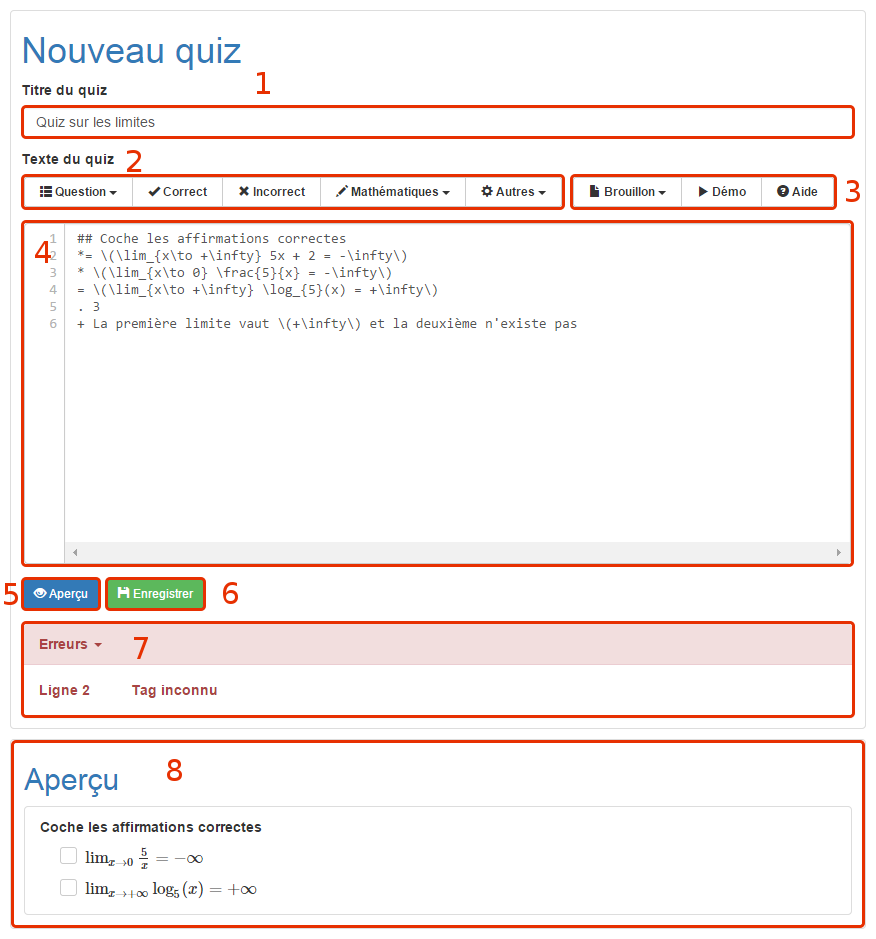
\includegraphics{create.png}
\end{figure}

Les professeurs peuvent créer un quiz en utilisant un format texte de type Markdown pour créer différents types de questions et y attribuer certaines caractéristiques. Cet éditeur de quiz se présente se présente sous la forme d'une zone de texte dans laquelle le professeur peut entrer le code du quiz. Au début de chaque ligne, le prof entre un tag pour préciser la fonction de la ligne, chaque tag a une signification différente. Le tag doit être séparé de la suite de la ligne par un espace.

\begin{tabulary}{\linewidth}{|L|L|}
\hline
\textsf{\relax 
Tag
} & \textsf{\relax 
Signification
}\\
\hline
\#\#
 & 
Question à choix multiple avec plusieurs options qui peuvent être choisies
\\

**
 & 
Question à choix multiple avec une seule option qui peut être choisie
\\

\textasciicircum{}\textasciicircum{}
 & 
Liste déroulante avec une option sélectionnable
\\

??
 & 
Question avec un champ de texte à remplir
\\

*
 & 
Option invalide dans un QCM
\\

=
 & 
Option valide dans un QCM
\\

=
 & 
Réponse correcte dans une question à champ de texte
\\

.
 & 
Permet de définir le nombre de points sur la question (par défaut, 1)
\\

+
 & 
Ajout d'un commentaire d'explication qui sera affiché lors de la correction
\\
\hline\end{tabulary}


Voici un exemple de quiz comprenant 4 questions :

\begin{Verbatim}[commandchars=\\\{\}]
\PYGZsh{}\PYGZsh{} Énoncé de la question à choix multiple (plusieurs cases peuvent être cochées)
* Option 1
* Option 2 (correcte)
* Option 3
* Option 4 (correcte)
+ Commentaire affiché à la correction
. 1.5

** Énoncé de la question à choix multiple (une seule case peut être cochée)
* Option 1
* Option 2
* Option 3 (correcte)
. 2

\PYGZca{}\PYGZca{} Liste déroulante
* Option 1
* Option 2 (correcte)
* Option 3
* Option 4

?? Question à champ de texte
* Réponse correcte
* Autre réponse correcte possible
\end{Verbatim}

Lorsque le professeur appuie sur le bouton \emph{Aperçu}, il peut voir le rendu du quiz tel que le verront les étudiants. Les éventuelles erreurs dans le code (tag qui n'existe pas, etc.) sont affichés en rouge en dessous de l'aperçu. Le quiz ne peut pas être enregistré tant qu'il y a encore des erreurs dans le code. S'il commence à créer un quiz et désire le terminer plus tard, le professeur peut enregistrer un brouillon. L'outil de création de quiz supporte l'affichage des mathématiques avec MathJax (\href{http://www.mathjax.org/}{http://www.mathjax.org/}).

Le prof doit également donner un titre au quiz et peut le relier à un ou plusieurs chapitres. Il décide de restreindre l'accès aux membres d'un ou plusieurs groupes ou de le rendre public. Pour créer un quiz, un prof a aussi la possibilité de reprendre un quiz déjà existant et de modifier son code. S'il opte pour cette solution, les statistiques du nouveau quiz ainsi créé repartent à zéro, puisque les questions ne sont plus forcément les mêmes.


\subsection{Consultation des statistiques avancées}
\label{functionalities:consultation-des-statistiques-avancees}
Après que les élèves d'un groupe ont complété un quiz, le professeur peut afficher le résultat moyen des élèves, le \% de réussite à chaque question, mais aussi les réponses soumises par chaque élève en particulier. Le prof peut ainsi se faire une idée globale et plus ciblée du niveau de compréhension de son groupe.


\section{Étudiants}
\label{functionalities:etudiants}

\subsection{Trouver un quiz}
\label{functionalities:trouver-un-quiz}\begin{figure}[htbp]
\centering

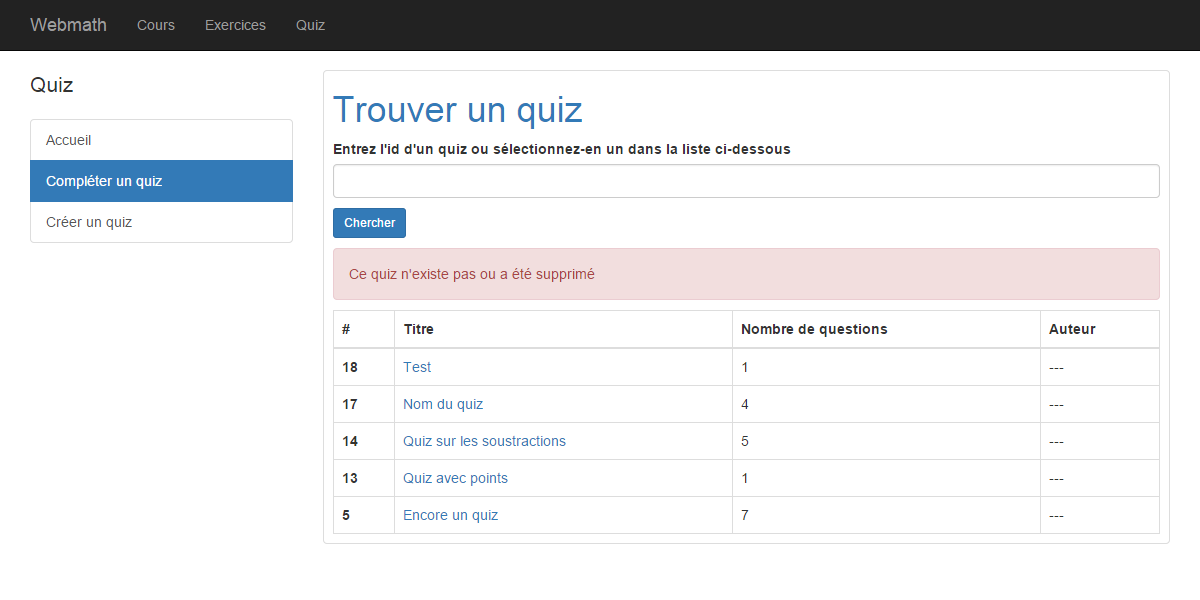
\includegraphics{find.png}
\end{figure}

Pour trouver un quiz, un étudiant a plusieurs possibilités. Le professeur peut donner l'url exacte du quiz à compléter, ce qui peut être pratique dans un e-mail ou toute communicaton informatisée. Une fonctionnalité permet au utilisateurs de générer un code QR correspondant à un quiz, ce qui est idéal pour afficher sur un projecteur en classe ou sur une feuille imprimée. Un étudiant peut aussi accéder à un quiz en mémorisant son id et en l'entrant dans la champ prévu à cet effet sur la page ``Trouver un quiz''.

Dans son espace utilisateur, l'étudiant peut aussi consulter les derniers quizs créés dans son groupe et peut donc y accéder facilement (fonctionnalité externe à l'application).


\subsection{Compléter un quiz et correction automatique}
\label{functionalities:completer-un-quiz-et-correction-automatique}
Une fois que l'étudiant à accédé au quiz, il peut le compléter très simplement en remplissant les champs de formulaires affichés. Lorsqu'il a fini, il peut soumettre ses réponses et il est redirigé vers une page de correction. Les réponses incorrectes sont affichées en rouge avec la solution et une explication pour chaque question. Les points reçus pour chaque question sont affichés avec le total de points sur le quiz. L'étudiant peut aussi comparer son score à la moyenne des autres étudiants du groupe. Un champ de texte est disponible pour envoyer des éventuelles remarques au professeur (signaler une erreur, poser une question). La page pour compléter un quiz ainsi que celle de la correction sont optimisées pour mobile et le design responsive s'adapte parfaitement à tous types de périphériques (ordinateur de bureau, ordinateur portable, tablette, téléphone mobile).
\begin{figure}[htbp]
\centering

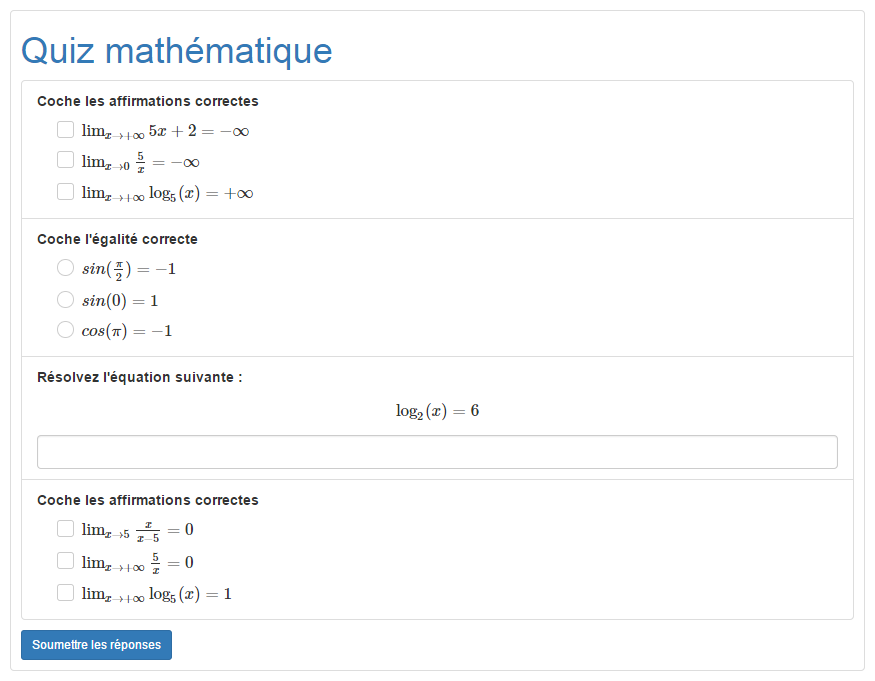
\includegraphics{complete.png}
\end{figure}


\chapter{Modèle relationnel}
\label{database:modele-relationnel}\label{database::doc}

\section{Introduction}
\label{database:introduction}
Une des premières étapes importantes dans le développement d'un site web est l'élaboration d'un modèle relationnel structuré permettant de stocker toutes les données générées par l'application et de les relier entre elles. Un modèle relationnel décrit les différentes tables de la base de donnée et les liens entre ces tables. Une table peut être comparée à un tableau contenant des informations. Chaque table comporte une ou plusieurs colonnes, chaque colonne stockant un type de données précisément défini (par exemple, un nombre entier ou une chaîne de caractères). Si on imagine une table contenant les données sur les utilisateurs d'un site, une colonne pourrait alors contenir le pseudonyme d'un utilisateur et une autre son âge. On peut ensuite ajouter des lignes à une table, c'est à dire un ensemble de données dont chaque élément correspond à une colonne de la table. Dans l'exemple précédent, on ajouterait ainsi une ligne pour chaque utilisateur s'inscrivant sur le site. Chaque ligne est identifiée grâce à une clé primaire unique, habituellement sous la forme d'un entier, qui permet de créer des liens entre différentes lignes de différentes tables (appelées relations).

Voici, présenté sous forme simplifiée à l'aide d'un tableau, comment on pourrait stocker les données concernant des quiz ainsi que leurs créateurs :

\textbf{Table contenant les utilisateurs :}

\begin{tabulary}{\linewidth}{|L|L|L|}
\hline
\textsf{\relax 
Clé primaire
} & \textsf{\relax 
Prénom
} & \textsf{\relax 
Âge
}\\
\hline
1
 & 
Paul
 & 
26
\\

2
 & 
Juliette
 & 
22
\\

3
 & 
Marc
 & 
48
\\
\hline\end{tabulary}


\textbf{Table contenant les quiz :}

\begin{tabulary}{\linewidth}{|L|L|L|L|}
\hline
\textsf{\relax 
Clé primaire
} & \textsf{\relax 
Titre du quiz
} & \textsf{\relax 
Nombre de questions
} & \textsf{\relax 
Auteur
}\\
\hline
1
 & 
Fonctions exponentielles
 & 
5
 & 
3
\\

2
 & 
Logarithmes
 & 
9
 & 
3
\\

3
 & 
Comportement à l'infini
 & 
8
 & 
2
\\
\hline\end{tabulary}


Ici, le premier quiz a comme titre \emph{Fonctions exponentielles}, comporte 5 questions et a été créé par Marc (Utilisateur 3).

Une fois que le modèle relationnel a été élaboré, on peut créer une base de données sous forme de fichier. Le langage SQL permet de créer les tables d'une base de données, d'y enregistrer des informations et de faire des requêtes (c'est à dire récupérer des données enregistrées). Un logiciel ou une application web peut ainsi communiquer avec une base de données et stocker les informations nécessaires de manière permanente.

Django offre la possibilité de créer une base de données et d'interagir celle-ci par le biais d'une API, on peut donc éviter l'utilisation du langage SQL et communiquer avec la base de données avec des objets et des méthodes Python.


\section{Utilisation dans l'application de création de quiz}
\label{database:utilisation-dans-l-application-de-creation-de-quiz}

\subsection{Implémentation dans Django}
\label{database:implementation-dans-django}
Comme indiqué précédemment, Django fournit une interface de haut niveau pour créer et interagir avec une base de données. On peut écrire nos tables avec une architecture orientée objet, que Django ``traduira'' ensuite en SQL. Ainsi, pour créer une table dans notre base de données, il suffit de définir une classe héritant de \code{models.Model} et d'initialiser des variables de classes pour ajouter des colonnes à la tables. Ainsi, par exemple, pour implémenter une table contenant les données générales d'un quiz, il suffit d'écrire le code suivant :

\begin{Verbatim}[commandchars=\\\{\}]
\PYG{k}{class} \PYG{n+nc}{Quiz}\PYG{p}{(}\PYG{n}{models}\PYG{o}{.}\PYG{n}{Model}\PYG{p}{)}\PYG{p}{:} \PYG{c}{\PYGZsh{}Infos générales sur le quiz}
    \PYG{n}{title} \PYG{o}{=} \PYG{n}{models}\PYG{o}{.}\PYG{n}{CharField}\PYG{p}{(}\PYG{n}{max\PYGZus{}length}\PYG{o}{=}\PYG{l+m+mi}{100}\PYG{p}{)} \PYG{c}{\PYGZsh{}Colonne contenant une chaîne de caractères}
    \PYG{n}{creation\PYGZus{}date} \PYG{o}{=} \PYG{n}{models}\PYG{o}{.}\PYG{n}{DateTimeField}\PYG{p}{(}\PYG{p}{)} \PYG{c}{\PYGZsh{}Colonne contenant une date/heure}
    \PYG{n}{code} \PYG{o}{=} \PYG{n}{models}\PYG{o}{.}\PYG{n}{CharField}\PYG{p}{(}\PYG{n}{max\PYGZus{}length}\PYG{o}{=}\PYG{l+m+mi}{1000}\PYG{p}{)} \PYG{c}{\PYGZsh{}Colonne contenant une chaîne de caractères}
\end{Verbatim}

Les fonctions comme \code{CharField()} ou \code{DateTimeField()} permettent de définir des champs d'un type de données précis. Une liste complète des types de champs est disponible sur la documentation officielle de Django : \href{https://docs.djangoproject.com/en/1.7/ref/models/fields/\#field-types}{https://docs.djangoproject.com/en/1.7/ref/models/fields/\#field-types}


\subsection{Schéma global}
\label{database:schema-global}
L'élaboration d'un schéma relationnel n'est pas chose facile car il est nécessaire que celui ci réponde à certains critères. Il doit être relativement simple afin de garder une certaine flexibilité et d'avoir la possiblité d'être modifié plus tard, car il est souvent difficile de prédire à l'avance les difficultés liées au stockage des données qui pourraient être rencontrées au cours du développement. Il doit également être possible d'ajouter des fonctionnalités sans devoir revoir toute l'organisation du schéma ou créer un trop grand nombre de nouvelles tables. Malgré cela, le modèle doit aussi correspondre aux exigences des fonctionnalités de l'application et doit inclure toutes les relations nécessaires. Il s'agit donc d'une étape cruciale qui peut s'avérer décisive pour la suite du développement.

Voici le diagramme des tables utilisés pour stocker les données des quiz :
\begin{figure}[htbp]
\centering

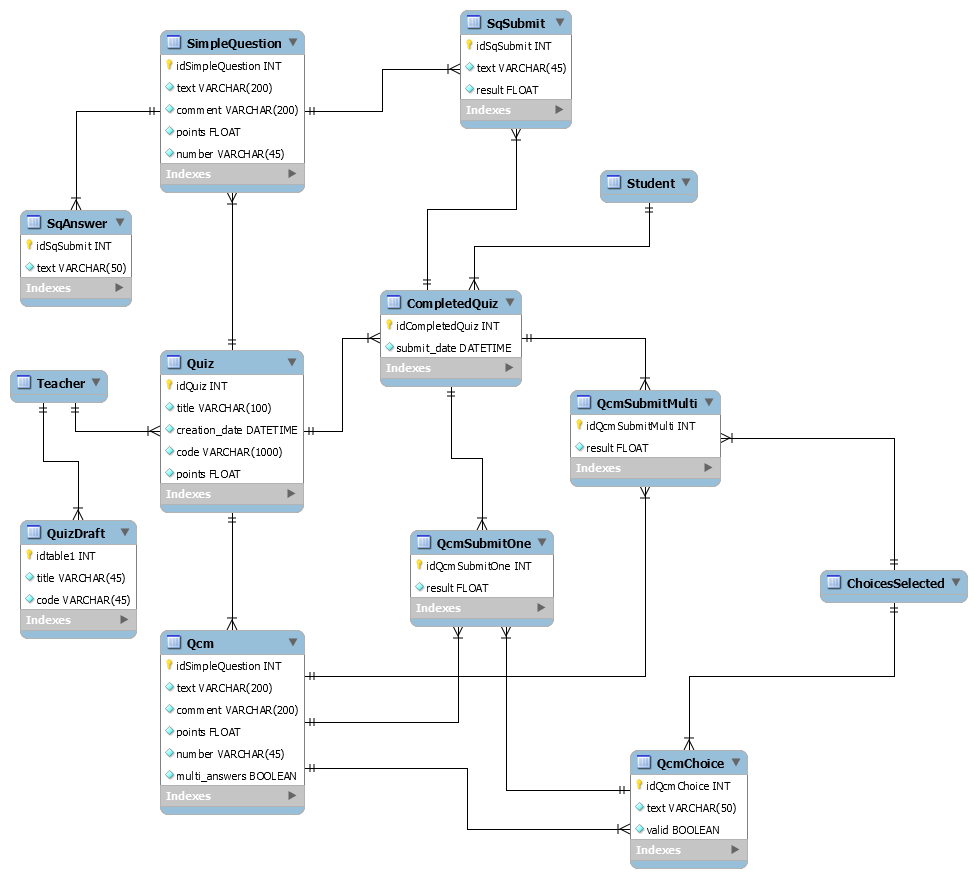
\includegraphics{quiz-models.png}
\end{figure}


\subsection{Explications des tables}
\label{database:explications-des-tables}

\subsubsection{Quiz}
\label{database:quiz}
La table \emph{Quiz} est la table centrale de l'application et toutes les autres tables s'organisent autour d'elle. Elle comporte trois colonnes : une contenant le titre, une autre contenant la date et l'heure de création (ajouté automatiquement lorsqu'un nouveau quiz est créé) ainsi qu'une colonne dans laquelle est stockée le code du quiz. L'intérêt de stocker ce code n'est pas forcément évident. Il est stocké afin de permettre à un professeur de créer un nouveau quiz à partir d'un quiz créé précédemment par lui-même ou un autre professeur (à condition que celui-ci l'ait rendu public). Le code peut ainsi être modifé pour ajouter des questions ou apporter une quelconque modification. Cette table comporte également une relation vers une table Teacher (qui ne fait pas partie de l'application de quiz) qui permet l'intégration dans le projet de groupe.

\textbf{Note :} la fonction de récupération de quiz existants n'est pas encore fonctionnelle.

Avec django, il est possible d'initialiser automatiquement un champ \code{DateTimeField} à la date/heure du moment où le modèle est instancié avec le paramètre \code{auto\_now\_add}

\begin{Verbatim}[commandchars=\\\{\}]
\PYG{n}{creation\PYGZus{}date} \PYG{o}{=} \PYG{n}{models}\PYG{o}{.}\PYG{n}{DateTimeField}\PYG{p}{(}\PYG{n}{auto\PYGZus{}now\PYGZus{}add}\PYG{o}{=}\PYG{n+nb+bp}{True}\PYG{p}{)}
\end{Verbatim}


\subsubsection{SimpleQuestion}
\label{database:simplequestion}
Cette table contient les informations générales sur les questions simples du quiz. Ces questions sont présentées sous la forme d'un simple champ de texte lorsqu'un élève complète le quiz. Une première colonne \emph{title} stocke l'énoncé de la question, \emph{comment} permet d'inclure un commentaire affiché lors de la correction automatique du quiz (par exemple la démonstration d'une égalité), \emph{points} définit le nombre de points attribués sur cette question et \emph{number} enregistre l'ordre auquel doit apparaître la question dans le quiz. Une relation désigne le quiz qui intègre la question.


\subsubsection{SqAnswer}
\label{database:sqanswer}
Cette table contient simplement la solution de la question définie par la relation vers la table \emph{SimpleQuestion}. Il est important de noter qu'il peut y avoir plusieurs solutions possibles pour une question et c'est la raison pour laquelle la solution n'est pas simplement stockée dans une colonne de \emph{SimpleQuestion}.


\subsubsection{Qcm}
\label{database:qcm}
La table Qcm permet de stocker les informations générales à propos des questions à choix multiples. Ces questions sont affichées sous forme de boutons radio, de cases à cocher ou de liste déroulante.
Cette table reprend plusieurs colonnes de la table \emph{SimpleQuestion}. C'est pourquoi ces deux tables héritent en fait du même modèle dans django :

\begin{Verbatim}[commandchars=\\\{\}]
\PYG{k}{class} \PYG{n+nc}{QuizQuestion}\PYG{p}{(}\PYG{n}{models}\PYG{o}{.}\PYG{n}{Model}\PYG{p}{)}\PYG{p}{:} \PYG{c}{\PYGZsh{}Classe abstraite dont héritent toutes les questions}
    \PYG{n}{text} \PYG{o}{=} \PYG{n}{models}\PYG{o}{.}\PYG{n}{CharField}\PYG{p}{(}\PYG{n}{max\PYGZus{}length}\PYG{o}{=}\PYG{l+m+mi}{200}\PYG{p}{)} \PYG{c}{\PYGZsh{}Énoncé}
    \PYG{n}{comment} \PYG{o}{=} \PYG{n}{models}\PYG{o}{.}\PYG{n}{CharField}\PYG{p}{(}\PYG{n}{max\PYGZus{}length}\PYG{o}{=}\PYG{l+m+mi}{200}\PYG{p}{,} \PYG{n}{blank}\PYG{o}{=}\PYG{n+nb+bp}{True}\PYG{p}{)} \PYG{c}{\PYGZsh{}Commentaire}
    \PYG{n}{points} \PYG{o}{=} \PYG{n}{models}\PYG{o}{.}\PYG{n}{FloatField}\PYG{p}{(}\PYG{n}{default}\PYG{o}{=}\PYG{l+m+mi}{1}\PYG{p}{)}
    \PYG{n}{number} \PYG{o}{=} \PYG{n}{models}\PYG{o}{.}\PYG{n}{IntegerField}\PYG{p}{(}\PYG{p}{)} \PYG{c}{\PYGZsh{}Ordre de la question dans le quiz}
    \PYG{n}{id\PYGZus{}quiz} \PYG{o}{=} \PYG{n}{models}\PYG{o}{.}\PYG{n}{ForeignKey}\PYG{p}{(}\PYG{n}{Quiz}\PYG{p}{)}

    \PYG{k}{class} \PYG{n+nc}{Meta}\PYG{p}{:}
        \PYG{n}{abstract} \PYG{o}{=} \PYG{n+nb+bp}{True}

\PYG{k}{class} \PYG{n+nc}{SimpleQuestion}\PYG{p}{(}\PYG{n}{QuizQuestion}\PYG{p}{)}\PYG{p}{:}
    \PYG{k}{pass} \PYG{c}{\PYGZsh{}Cette table reprend simplement les mêmes colonnes que le modèle abstrait}

\PYG{k}{class} \PYG{n+nc}{Qcm}\PYG{p}{(}\PYG{n}{QuizQuestion}\PYG{p}{)}\PYG{p}{:}
    \PYG{n}{multi\PYGZus{}answers} \PYG{o}{=} \PYG{n}{models}\PYG{o}{.}\PYG{n}{BooleanField}\PYG{p}{(}\PYG{p}{)}
    \PYG{n}{show\PYGZus{}list} \PYG{o}{=} \PYG{n}{models}\PYG{o}{.}\PYG{n}{BooleanField}\PYG{p}{(}\PYG{p}{)}
\end{Verbatim}

En plus des colonnes héritées, \emph{Qcm} possède deux champs de types booléens : \emph{multi\_answers}, qui définit si plusieurs options peuvent être cochées ou non, et \emph{show\_list}, qui vaut \code{True} si la question est affichée sous forme de liste déroulante. Si plusieurs options peuvent être cochées, la question sera dans tous les cas affichée à l'aide de cases à cocher.


\subsubsection{QcmChoice}
\label{database:qcmchoice}
Cette table contient les différents choix possibles pour la question définie par la relation vers \emph{Qcm}. Elle est formée de deux champs, le premier contenant le texte du choix et l'autre définissant par un booléen s'il est correct ou non de cocher ce choix. Une question à choix multiples doit avoir au moins deux choix possibles et au moins un choix correct. Si \emph{multi\_answers} vaut \code{False} dans \emph{Qcm}, une seule option peut être correcte puisque l'étudiant n'a la possibilité de cocher qu'une seule option.

\textbf{Note :} D'un point de vue purement relationnel, comme il est indiqué sur le diagramme, cette table possède une relation vers une table qui sert d'intermédiaire entre \emph{QcmChoice} et \emph{QcmSubmitMulti}. Cette table intermédiaire crée en fait une relation de type \emph{many-to-many}. L'implémentation de ce type de relation avec Django sera abordé plus loin.


\subsubsection{CompletedQuiz}
\label{database:completedquiz}
Comme on peut le voir sur le diagramme, à l'instar de \emph{Quiz}, cette table occupe aussi un rôle central dans le modèle relationnel. Elle permet de faire le lien entre un quiz créé par un professeur et les réponses soumises à ce quiz par les étudiants. Elle possède donc une relation vers une table \emph{Student} (encore une fois extérieure à l'application). De l'autre côté, cette table pointe vers \emph{Quiz} et définit logiquement le quiz auquel l'étudiant a répondu. Un seul champ est présent : la date et l'heure de la soumission des réponses.


\subsubsection{SqSubmit}
\label{database:sqsubmit}
Il s'agit simplement de la réponse apportée à une question simple. La table a donc un champ \emph{text} qui contient la réponse soumise par l'élève. Elle possède aussi deux relations, une vers \emph{SimpleQuestion} pour préciser la question auquel l'élève a répondu, et une autre vers \emph{CompletedQuiz}. La réponse soumise par l'élève sera ensuite comparée à(aux) solution(s) enregistrées pour déterminer si les points sont attribués ou non.


\subsubsection{QcmSubmitOne et QcmSubmitMulti}
\label{database:qcmsubmitone-et-qcmsubmitmulti}
Ces deux tables sont très similaires. \emph{QcmSubmitOne} contient une relation vers l'option sélectionnée par l'étudiant dans une question à choix multiples avec \emph{multi\_answers} valant \code{False}, tandis que \emph{QcmSubmitMulti} peut contenir des relations vers plusieurs options, quand \emph{multi\_answers} vaut \code{True}. Il s'agit donc dans le premier cas d'une relation \emph{many-to-one}, puique plusieurs lignes (réponses fournies par différents élèves) peuvent pointer vers la même option. Dans le deuxième cas, c'est une relation de type \emph{many-to-many}, puisque plusieurs lignes peuvent pointer vers plusieurs options.

Dans Django, voici comment seront définies ces relations :

\begin{Verbatim}[commandchars=\\\{\}]
\PYG{n}{id\PYGZus{}selected} \PYG{o}{=} \PYG{n}{models}\PYG{o}{.}\PYG{n}{ForeignKey}\PYG{p}{(}\PYG{n}{QcmChoice}\PYG{p}{,} \PYG{n}{null}\PYG{o}{=}\PYG{n+nb+bp}{True}\PYG{p}{)} \PYG{c}{\PYGZsh{}Relation many\PYGZhy{}to\PYGZhy{}one}
\PYG{n}{id\PYGZus{}selected} \PYG{o}{=} \PYG{n}{models}\PYG{o}{.}\PYG{n}{ManyToManyField}\PYG{p}{(}\PYG{n}{QcmChoice}\PYG{p}{,} \PYG{n}{null}\PYG{o}{=}\PYG{n+nb+bp}{True}\PYG{p}{)} \PYG{c}{\PYGZsh{}Relation many\PYGZhy{}to\PYGZhy{}many}
\end{Verbatim}

L'argument \code{null} vaut ici \code{True} car il se peut que l'étudiant ne coche aucun choix. Dans ce cas-là, il n'obtiendra dans tous les cas aucun point.



\renewcommand{\indexname}{Index}
\printindex
\end{document}
